\PassOptionsToPackage{table}{xcolor}
\documentclass{cernatsnote}
\usepackage[colorinlistoftodos]{todonotes}
\usepackage{placeins}
\usepackage{float}
\usepackage{rotating}
\usepackage{verbatim}
\usepackage{fancyvrb}
\usepackage{listings}
\lstdefinestyle{python}{
  language=Python,
  basicstyle=\small\ttfamily,
  keywordstyle=\color[RGB]{0,0,200}\bfseries,
  stringstyle=\color[RGB]{163,21,21},
  commentstyle=\color[RGB]{0,128,0}\itshape, 
  numberstyle=\tiny\color{gray},
  backgroundcolor=\color{codebg},
  frame=single,
  framerule=0.4pt,
  rulecolor=\color{framecolor},
  showstringspaces=false,
  breaklines=true,
  morekeywords={True,False,None},
}
\lstdefinestyle{tcl}{
  language=tcl,
  basicstyle=\small\ttfamily,
  keywordstyle=\color[RGB]{0,0,200}\bfseries,
  stringstyle=\color[RGB]{163,21,21},
  commentstyle=\color[RGB]{0,128,0}\itshape,
  numberstyle=\tiny\color{gray},
  backgroundcolor=\color{codebg},
  frame=single,
  framerule=0.4pt,
  rulecolor=\color{framecolor},
  showstringspaces=false,
  breaklines=true,
}
\usepackage[T1]{fontenc}
\usepackage{graphicx}
\graphicspath{{images/}}
\usepackage{xcolor}
\usepackage{colortbl}
\usepackage{booktabs}
\usepackage{longtable}
\usepackage{multirow}
\usepackage{array}
\definecolor{codebg}{RGB}{245,245,245}
\definecolor{framecolor}{RGB}{180,180,180}
\definecolor{darkgreen}{RGB}{0,128,0}
% Register map colors
\definecolor{rwgreen}{RGB}{15,110,86}
\definecolor{rwbg}{RGB}{225,245,238}
\definecolor{roblue}{RGB}{24,95,165}
\definecolor{robg}{RGB}{230,241,251}
\definecolor{woamber}{RGB}{133,79,11}
\definecolor{wobg}{RGB}{250,238,218}
\definecolor{headerbg}{RGB}{241,239,232}
\definecolor{sectionbg}{RGB}{230,230,230}
\definecolor{monocolor}{RGB}{60,52,137}
% Register map badge commands
\newcommand{\badrw}{\colorbox{rwbg}{\textcolor{rwgreen}{\textbf{\small R/W}}}}
\newcommand{\badro}{\colorbox{robg}{\textcolor{roblue}{\textbf{\small RO}}}}
\newcommand{\badwo}{\colorbox{wobg}{\textcolor{woamber}{\textbf{\small WO}}}}
\newcommand{\reg}[1]{\texttt{\textcolor{monocolor}{#1}}}
\newcommand{\addr}[1]{\texttt{\small #1}}
\newcolumntype{L}[1]{>{\raggedright\arraybackslash}p{#1}}
\newcolumntype{C}[1]{>{\centering\arraybackslash}p{#1}}
\newcommand{\subrow}[1]{\rowcolor{sectionbg} \multicolumn{5}{l}{\small\textbf{\textsc{#1}}} \\}

\title{DFX4ML-ARCH (Progress Update)}
\author{
	Omitted for blind review \\
	CERN, CH-1211 Geneva, Switzerland
}
\email{Tanawin1701d@outlook.com}
\date{\today}

\begin{document}
\maketitle

\begin{abstract}
DFX4ML-ARCH presents an FPGA architecture designed to enable partial reconfiguration for machine learning workloads. The project incorporates a self-reconfiguration mechanism, allowing the FPGA fabric to partially reprogram itself. It targets AMD FPGAs equipped with the ICAP3 interface and leverages the PYNQ framework for system integration.
\end{abstract}
\\ \\ \\

\begin{small}
\noindent\textbf{Disclaimer:} The technical content, architecture designs, implementation decisions, and all intellectual contributions in this report are entirely the work of the authors. Generative AI tools were used solely for grammar correction and readability enhancement of the written text. No AI-generated technical content, code, or design decisions are included.

\medskip
\noindent\textbf{Template:} This document uses the CERN ATS Note \LaTeX{} template, available at \url{https://www.overleaf.com/latex/templates/cern-ats-note/yzjmgkrvtsqg}.
\end{small}

\bigskip

\begingroup
\color{black}
\tableofcontents
\endgroup

\pagebreak

\section{Introduction}

The goal of this experiment session is to gather empirical data on the key parameters that govern design trade-offs in an FPGA partial reconfiguration system for machine learning workloads. The results will inform architectural decisions going forward.

\subsection{Parameters Under Consideration}

\begin{description}
  \item[Data Batch Size]
    Varies with static region size and model I/O type.
    A larger batch size is desirable, but it competes directly with the desire for a large static region.

  \item[FPGA Static Region Size]
    Should be as small as possible to leave more area for the dynamic region.

  \item[FPGA Dynamic Region Size]
    Should be as large as possible to accommodate larger ML models.
    However, a larger dynamic region increases reconfiguration time.

  \item[Reconfiguration Time]
    Should be as small as possible, which pushes toward a smaller dynamic region --- directly opposing the goal above.

  \item[Model Size]
    Larger ML models are preferred, but they require a larger dynamic region, which increases reconfiguration time.

\end{description}

\subsection{Goal}

Quantify the actual trends between these parameters so that architectural decisions can be grounded in evidence rather than assumption. Three experiment sessions are proposed:

\begin{enumerate}

  \item \textbf{Region Size vs. Reconfigure Time} ---
    The reconfiguration time depends on the size of the dynamic region (\textbf{not the size of the model within the dynamic region}). The experiment aims to explore the trend in reconfiguration time across varying dynamic region sizes.

  \item \textbf{DFX Streamer Packing Exploration} ---
    We propose an optimised approach to expand the dynamic region as much as possible while retaining as much BRAM/URAM in the static region for the DFX Streamer as possible.

  \item \textbf{Latency Hiding Technique (IN PROGRESS)} ---
    We propose a technique to hide latency by using the double dynamic region method to keep the system executing continuously.


\end{enumerate}

With data from all sessions, the aim is to identify the operating point that maximises performance, or at minimum to establish a principled basis for deciding the next phase of the design.



\section{Architecture Upgrade}

\subsection{DFX Streamer}


\subsubsection{Problems}

We encountered 2 problems with Vivado and the KV260:

\begin{enumerate}
  \item \textbf{Vivado cannot handle a single large BRAM/URAM array.}
    Vivado synthesis rejects the \texttt{mainMem} variable in \texttt{dfx\_streamer.v} (line~82) with the following error:

    \begin{quote}
      \ttfamily\small
      [Synth 8-4556] size of variable `mainMem' is too large to handle; \\
      the size of the variable is 20{,}480{,}000, the limit is 1{,}000{,}000.
    \end{quote}

    The variable \texttt{mainMem} is declared as a flat Verilog register array whose total bit-width (20\,480\,000) exceeds Vivado's synthesis limit of 1\,000\,000 bits.
    Vivado cannot map such a monolithic array to physical BRAM/URAM primitives directly.
    The fix is to split \texttt{mainMem} into multiple smaller arrays, each within the 1\,000\,000-bit limit, so that Vivado can infer and place individual BRAM/URAM tiles.

  \item \textbf{Border Latency Problem}
    The old version of DFX Streamer (Magic Streamer) requires one cycle to save data to BRAM/URAM. The timing constraint is not met. The assumption is that placement restrictions across different Pblocks are responsible. Fig.~\ref{fig:bram_problem} illustrates the SRC signal (green block), which is constrained to the dynamic region, while the target BRAM spans another region. Vivado cannot perform fan-out optimisation across regions, especially the dynamic region. Moreover, Vivado cannot retime the path either.

    \begin{figure}[H]
      \centering
      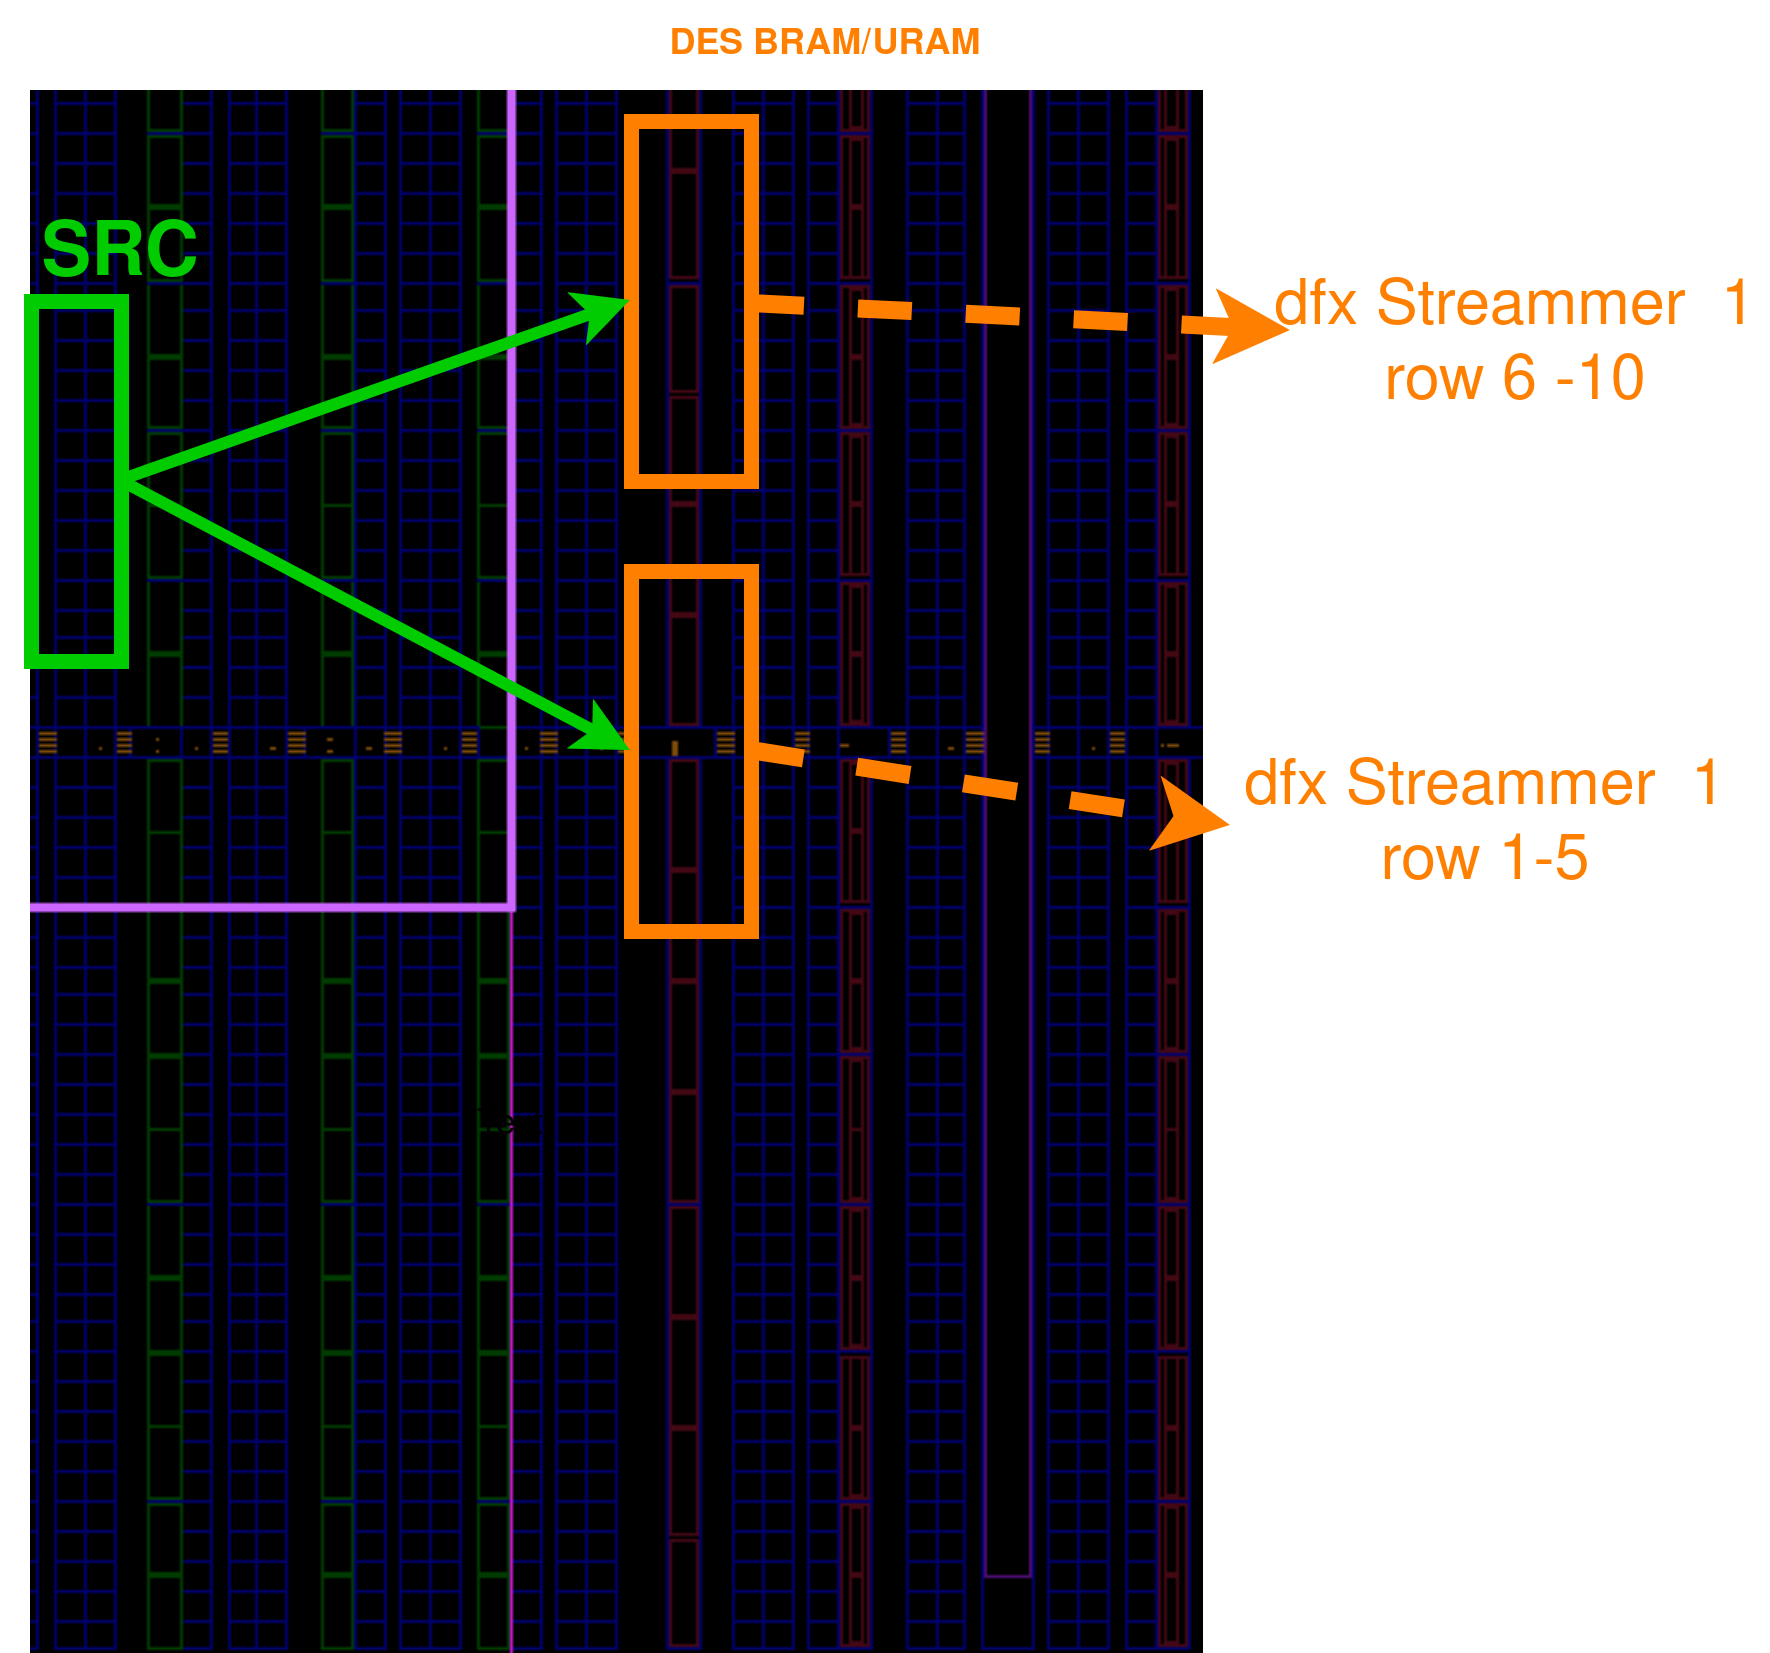
\includegraphics[width=0.55\linewidth]{bram_problem.png}
      \caption{Vivado synthesis error caused by oversized \texttt{mainMem} array in \texttt{dfx\_streamer.v}.}
      \label{fig:bram_problem}
    \end{figure}
 
\end{enumerate}
 
\subsubsection{DFX Stream Next Gen}

We address the DFX Streamer's problems by fully re-architecting the memory management system.

\begin{figure}[H]
  \centering
  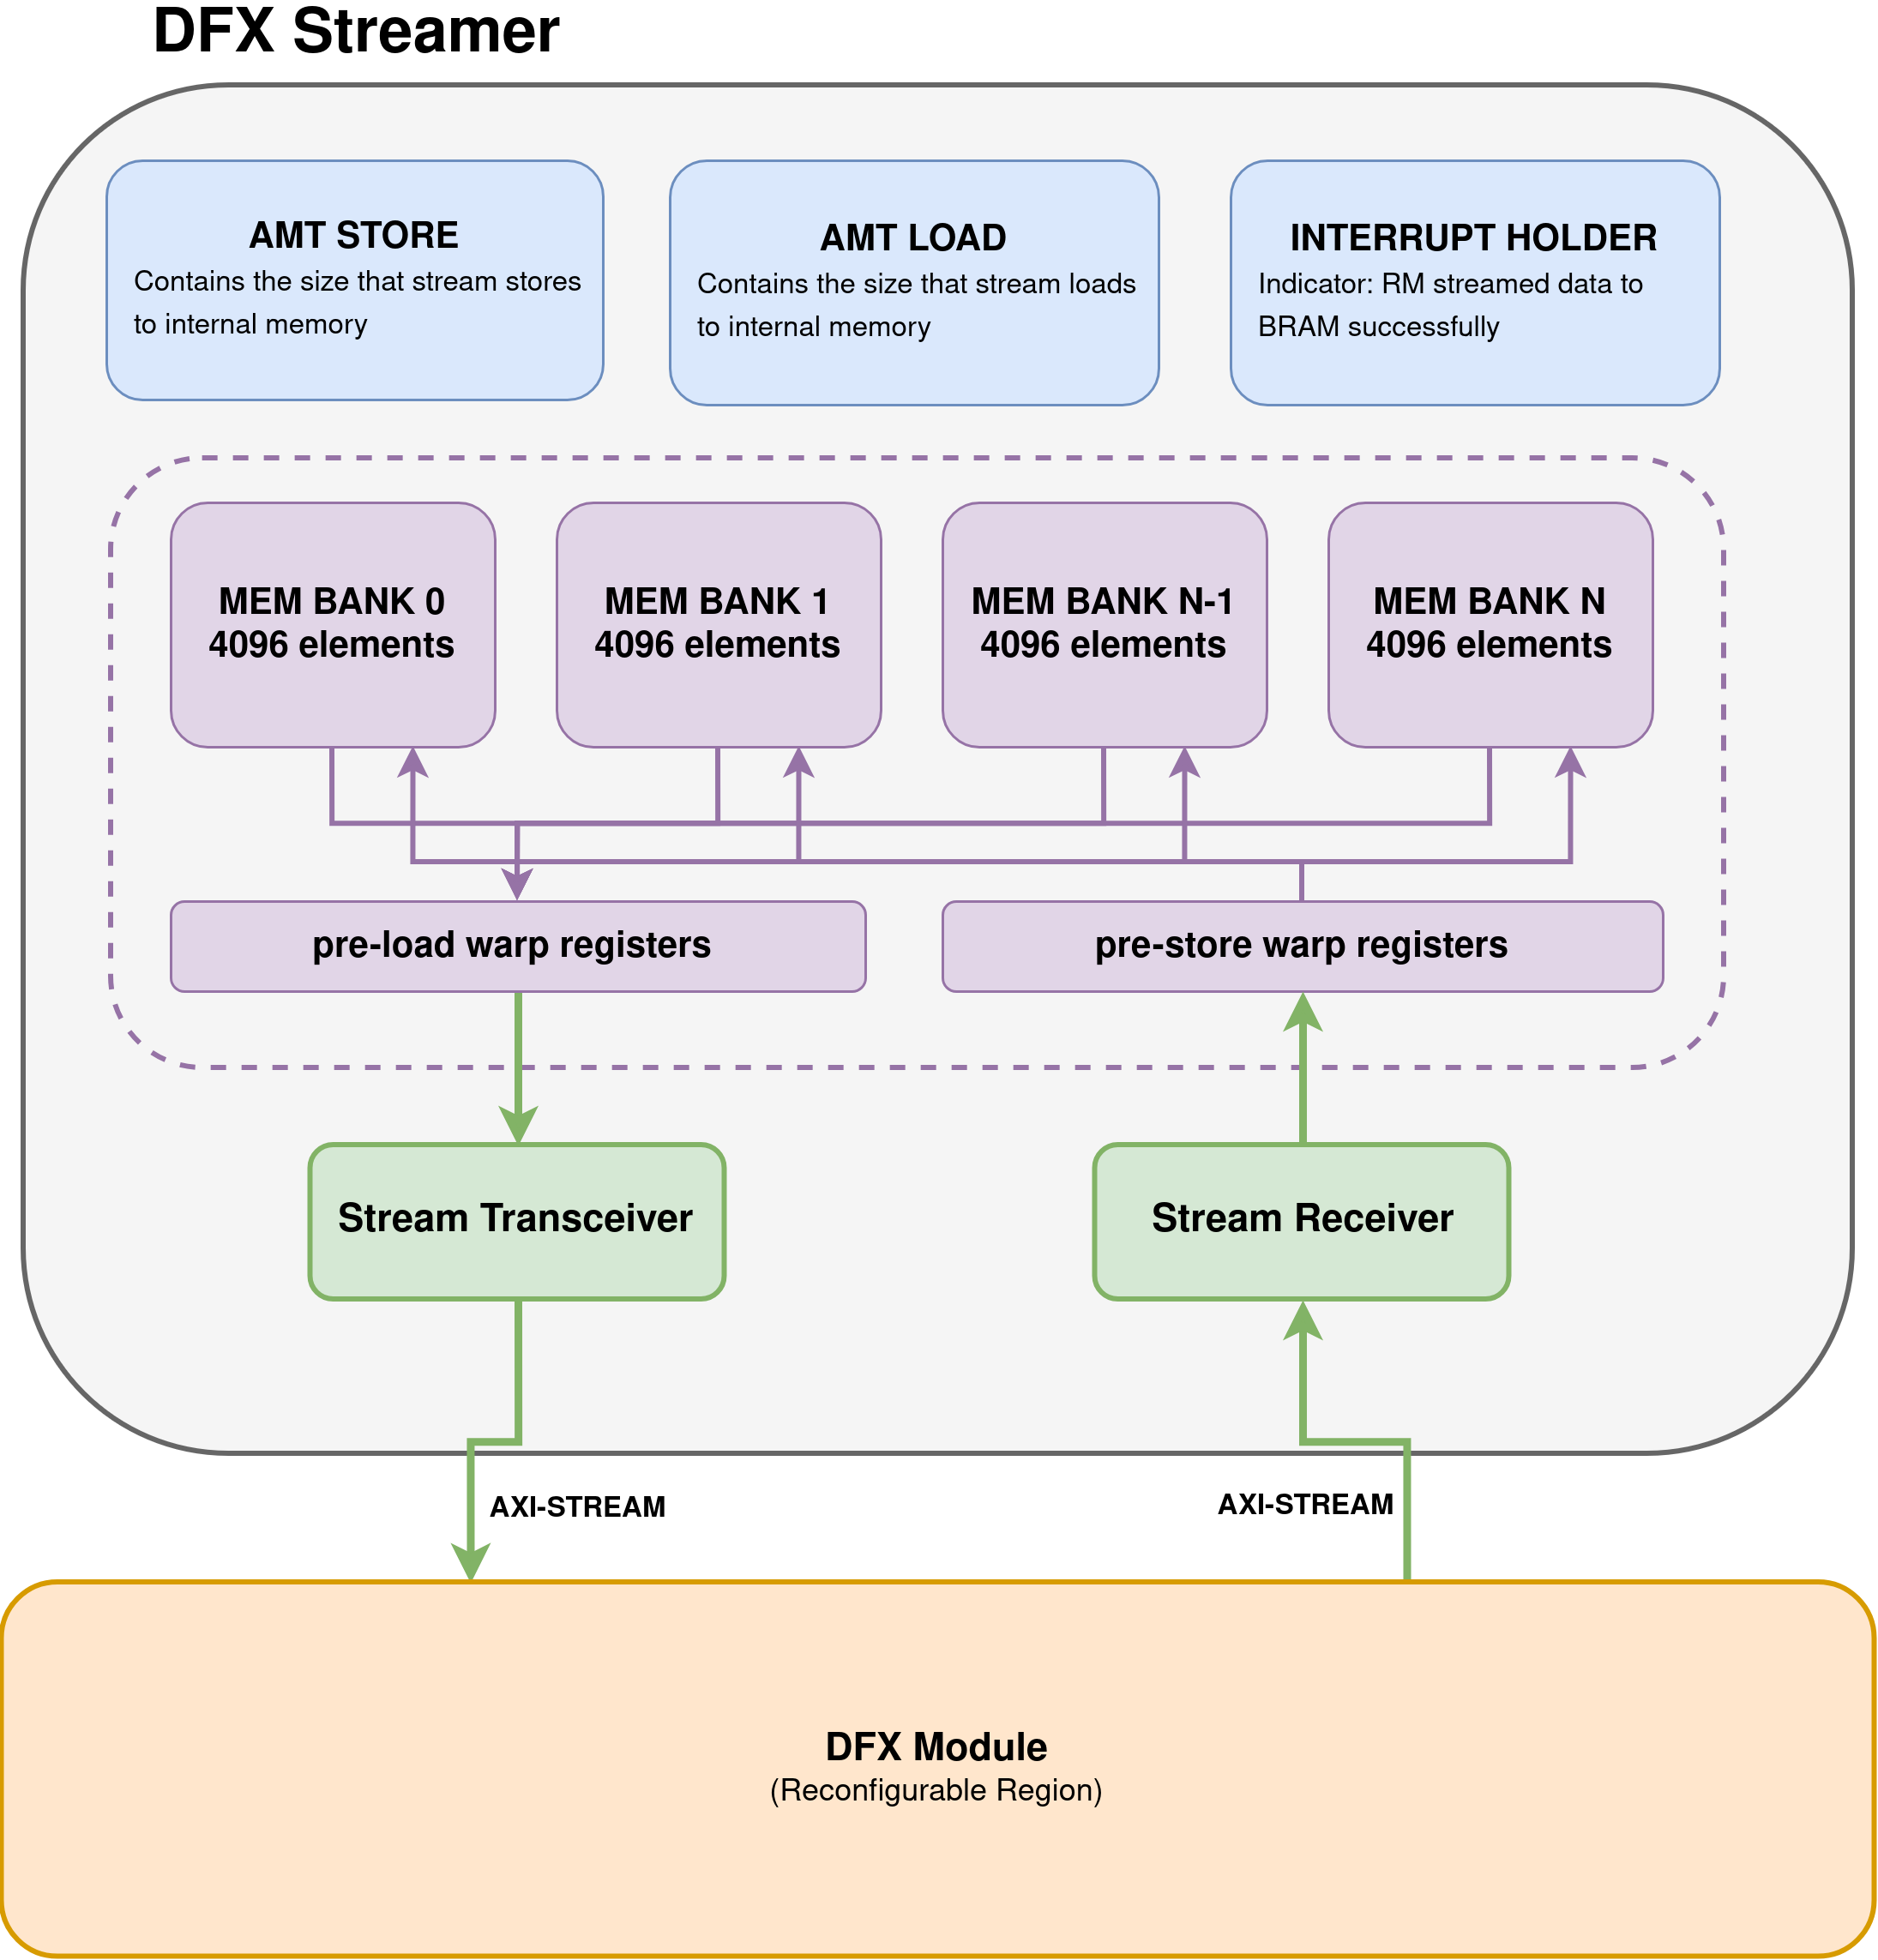
\includegraphics[width=0.65\linewidth]{dfx_streamer2.png}
  \caption{DFX Streamer next-generation architecture.}
  \label{fig:dfx_streamer2}
\end{figure}


First, to address the Vivado error, we divide the DFX Streamer's memory into multiple banks. Each bank has I/O equal to the I/O of the ML model's front wrap. However, a wrap width that is a multiple of 64 bits is recommended since the URAM's bit-width is 64 bits.

Moreover, the DFX Streamer packs 4096 entries per bank to maximise resource utilisation for each URAM. If entries are not packed, Vivado cannot decide to merge two memory banks into a single URAM/BRAM, even when they are not accessed simultaneously.

Second, to address the latency problem, we pipeline the URAM/BRAM data transfer (both load and store). On the store side, we add an additional register equal to the wrap size to buffer data coming from the dynamic region. On the load side, we add an additional register equal to $\text{wrap size} \times \text{number of memory banks}$; the pipeline supports back-pressure in case the ML model is not ready to receive data from the memory bank.


\subsection{DFX Manager Next Gen}

In the current experiment session, we used the ML model from HLS4ML's Vitis Unified Backend; therefore we need AXI-Lite to control the model. We have added two registers to BANK 0 of the \texttt{s\_axi\_write} module:

\begin{itemize}
  \item \textbf{Address DFX\_MAN\_ADDR + \texttt{0x240}} --- \reg{prCtrlAddr}: stores the base address of the PR control IP (AXI-Lite slave of the HLS4ML model).
  \item \textbf{Address DFX\_MAN\_ADDR + \texttt{0x280}} --- \reg{batchSize}: stores the batch size used for a single inference invocation.
\end{itemize}

Both registers are 32-bit wide (\texttt{GLOB\_ADDR\_WIDTH} / \texttt{GLOB\_DATA\_WIDTH}) and are decoded from address bits~[13:6] in the BANK~0 region (\texttt{write\_addr[15:14] == 2'b00}).

To accurately collect the execution time for each ML model, we added a 32-bit register to Bank 1 (\textbf{\texttt{0x4024 + 0x64 * RM\_ID}}) to record the number of elapsed cycles in the system.


\subsection{DFX Decoupler Controller Next Gen}

For debugging purposes, in the old version the DFX Controller IP owned the DFX decoupler, making it impossible for the PS to bypass control in some situations. We therefore redesigned the ownership control of the DFX decoupler, located at address \texttt{0xA001\_0000}. The register bit-field definition is shown in Table~\ref{tab:dfx_decoupler_reg}.

\begin{table}[H]
  \centering
  \caption{DFX Decoupler Control Register (\texttt{0xA001\_0000}) bit-field definition.}
  \label{tab:dfx_decoupler_reg}
  \begin{tabular}{C{1.2cm} C{1.6cm} C{2.2cm} p{8.2cm}}
    \toprule
    \textbf{Bit} & \textbf{Access} & \textbf{Value} & \textbf{Description} \\
    \midrule
    \multirow{2}{*}{0} & \multirow{2}{*}{\badwo} &

        \texttt{1} & Ownership of the DFX decoupler belongs to the \textbf{DFX Controller IP}. \\
    & & \texttt{0} & Ownership of the DFX decoupler belongs to the \textbf{PS} (Processing System). \\
    \midrule
    \multirow{2}{*}{1} & \multirow{2}{*}{\badwo} &

        \texttt{1} & Decouple~0 is \textbf{coupled} (active). Valid only when Bit~0~\texttt{= 0} (PS ownership). \\
    & & \texttt{0} & Decouple~0 is \textbf{decoupled}. Valid only when Bit~0~\texttt{= 0} (PS ownership). \\
    \bottomrule
  \end{tabular}
\end{table}

\pagebreak


\section{Temporal HLS4ML Vitis Unified Backend Modification}

To explore multiple designs that fit into DFX4ML and the KV260, we decided to modify the HLS4ML Vitis Unified backend to enable its interface to connect to the DFX4ML system. However, we did not want to build a full new backend at this stage. We wanted the minimal modifications as follows:

\begin{enumerate}
  \item The modified backend intermediates the layer's wrap as bare-metal bits (without converting back to float32 or another type).
  \item We use the software prediction result from the old Vitis Unified Backend for result checking.
  \item We use the FIFO-depth optimisation from the old Vitis Unified Backend and manually copy it into the new chopped model.
\end{enumerate}

\begin{sloppypar}
the modified backend is at \url{https://github.com/Tanawin1701d/hls4ml/tree/VitisUnifiedPartialExp}
\end{sloppypar}


\subsection{Interface Configuration}

The modified backend is invoked via the following call:

\begin{lstlisting}[style=python]
hls_model = hls4ml.converters.convert_from_keras_model(
    keras_model,
    hls_config=cfg,
    output_dir=output_dir,
    input_flat=input_flat,
    output_flat=output_flat,
    package_as_xo=full_run,
    project_name=_PROJECT_NAMES[key],
    **_HLS_PARAMS,
)
\end{lstlisting}
 
Three parameters are specific to the modified backend:

\begin{description}
  \item[\texttt{input\_flat}]
    A boolean flag that controls whether the model's input wrap is flattened into a 1-D stream of bare-metal bits before being passed to the HLS kernel.
    When \texttt{True}, the input is flattened; when \texttt{False}, the system converts from float32 to the target tensor type.

  \item[\texttt{output\_flat}]
    The output-side counterpart of \texttt{input\_flat}.

  \item[\texttt{package\_as\_xo}]
    When \texttt{True} (bound to \texttt{full\_run}), the backend runs the full new Vitis HLS flow and packages the resulting kernel as an \texttt{.xo} object file ready for linking.
    When \texttt{False}, the system follows the Vitis HLS IP flow for Vivado.
\end{description}

\begin{sloppypar}
The in detail implementation of the modified interface is at \url{https://github.com/Tanawin1701d/hls4ml/blob/VitisUnifiedPartialExp/hls4ml/templates/vitis_unified/myproject_axi_stream.cpp}
\end{sloppypar}

\pagebreak

\section{Experiment}

\subsection{Dynamic Region Size vs Reconfigure Time}

Two build projects were synthesised on the KV260 board (100\,MHz system clock) with
different dynamic-region sizes.
Table~\ref{tab:recon_raw} summarises the raw measurements.

\begin{table}[H]
  \centering
  \caption{Measured reconfiguration time for two dynamic-region configurations on KV260 (100\,MHz).}
  \label{tab:recon_raw}
  \small
  \begin{tabular}{lrrrr}
    \toprule
    \textbf{Project} & \textbf{Size (KB)} & \textbf{Recon.\ cycles} & \textbf{Recon.\ time (ms)} & \textbf{Throughput (MB/s)} \\
    \midrule
    \texttt{build\_prj\_0} & 1436 & 367\,778 & 3.678 & 381.4 \\
    \texttt{build\_prj\_1} & 2897 & 741\,674 & 7.417 & 381.5 \\
    \bottomrule
  \end{tabular}
\end{table}

\begin{figure}[H]
  \centering
  \begin{minipage}[t]{0.48\linewidth}
    \centering
    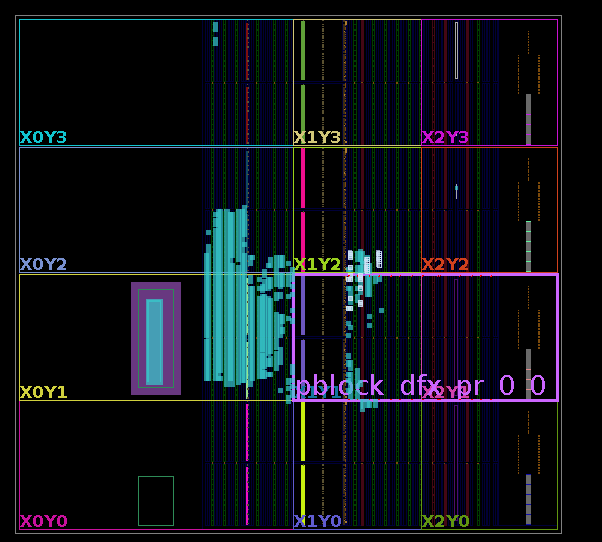
\includegraphics[width=\linewidth]{build_project_0.png}
    \caption{\texttt{build\_prj\_0} dynamic region.}
    \label{fig:build_prj_0}
  \end{minipage}
  \hfill
  \begin{minipage}[t]{0.48\linewidth}
    \centering
    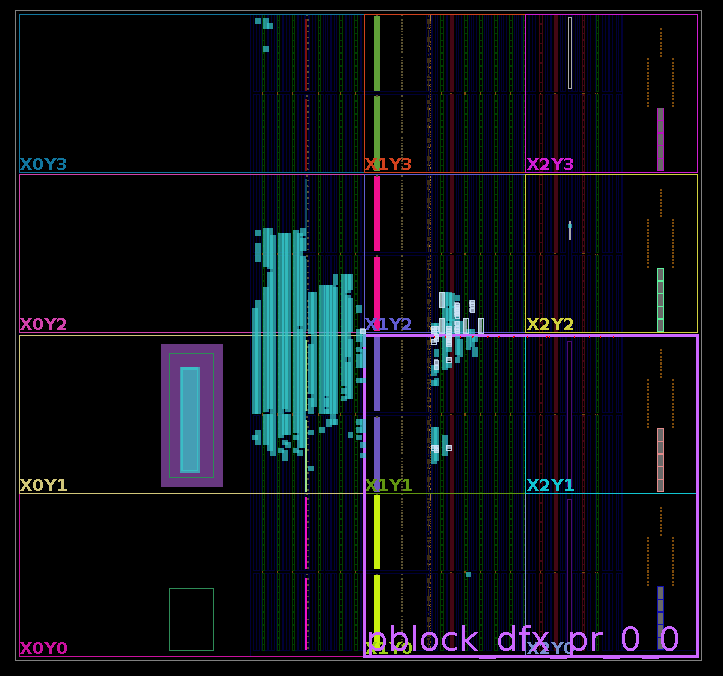
\includegraphics[width=\linewidth]{build_project_1.png}
    \caption{\texttt{build\_prj\_1} dynamic region.}
    \label{fig:build_prj_1}
  \end{minipage}
\end{figure}

The reconfiguration time is linear in bitstream size (ICAP3 throughput is constant at
$\approx$381\,MB/s), which yields the fitted model:
\[
  t_{\text{recon}}(\text{KB}) \;=\; 0.002560 \times \text{file\_size}_{\text{KB}} + 0.0010
  \quad [\text{ms}]
\]

Figure~\ref{fig:recon_bar} shows the per-project reconfiguration time and Figure~\ref{fig:recon_scatter} shows the linear relationship with predictions extrapolated up to a 22\,MB bitstream.

\begin{figure}[H]
  \centering
  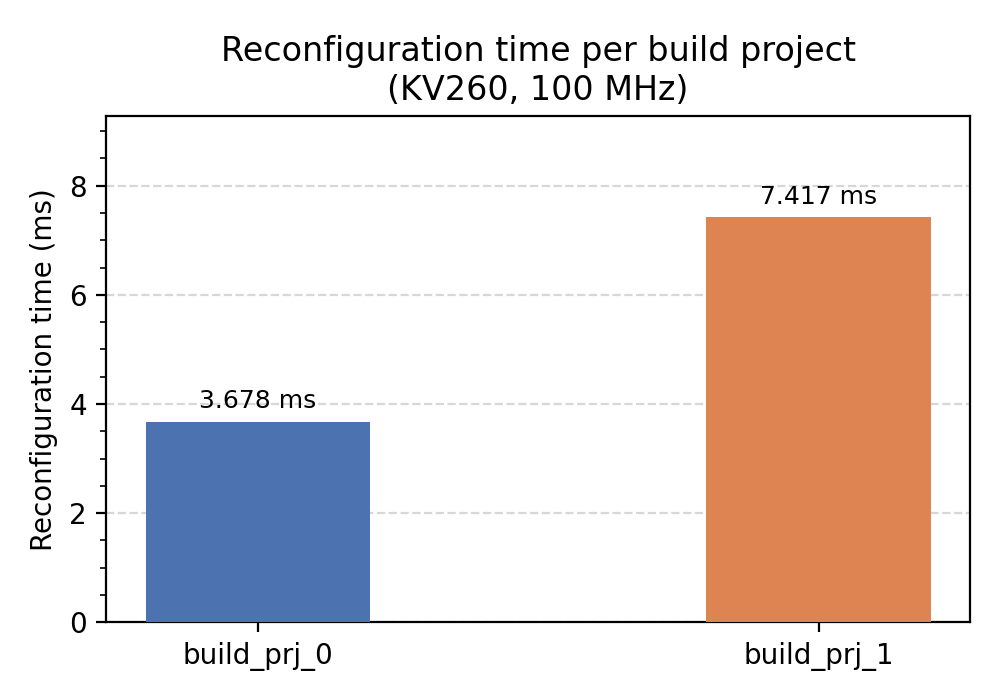
\includegraphics[width=0.55\linewidth]{recon_time_bar.png}
  \caption{Reconfiguration time per build project on KV260 (100\,MHz).}
  \label{fig:recon_bar}
\end{figure}

\begin{figure}[H]
  \centering
  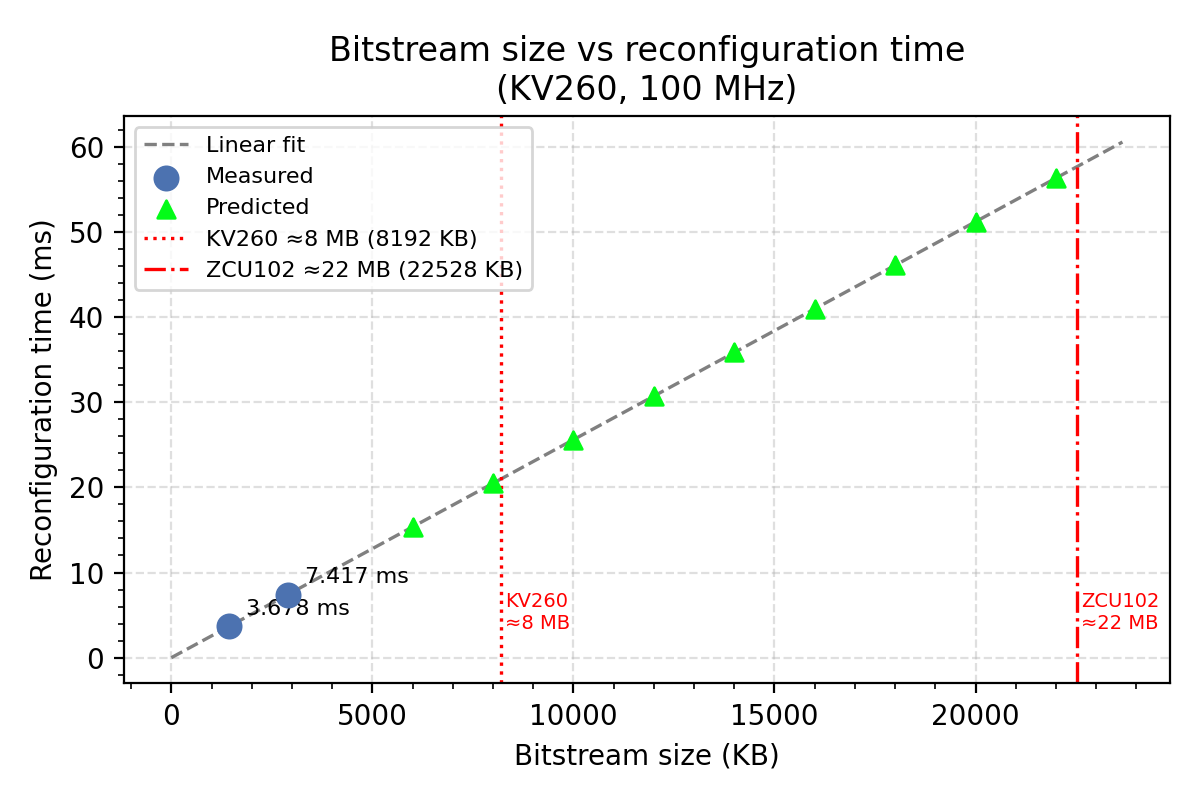
\includegraphics[width=0.72\linewidth]{recon_time_scatter.png}
  \caption{Bitstream file size vs.\ reconfiguration time with linear fit and predictions up to 22\,MB.}
  \label{fig:recon_scatter}
\end{figure}

\textbf{Key Takeaway}: As previously observed in experiments on the ZCU102, the reconfiguration rate is limited to $\sim$399\,MB/s; the bottleneck is the ICAP3 port, which accepts only 32 bits per cycle (4 bytes). At 100\,MHz, the throughput therefore saturates at 400\,MB/s (4 bytes $\times$ 100\,MHz).

In addition, the bitstream file size and reconfiguration time do not depend on the number of used logic cells in the FPGA; they depend only on the region size in the fabric.
 
\pagebreak

\subsection{DFX Streamer Packing Exploration}


\subsubsection{Dynamic Region Layout}

We allocate the fabric's resources between the dynamic region and the static region as follows.

\begin{enumerate}
  \item Static Region: we need it as small as possible since it is not directly involved in ML workloads. However, we require as much on-chip memory as possible, since the DFX Streamer uses it to hold intermediate data.
  \item Dynamic Region: we need it as large as possible since it is primarily used for ML workloads. However, a larger region may encroach on the static region's URAM/BRAM and increase reconfiguration time.
\end{enumerate}




As a result, we design the region arrangement shown in Fig.~\ref{fig:packing_layout}.
We compact the static region into the right side of the fabric, which has abundant URAM/BRAM resources.
Table~\ref{tab:static_mem} summarises the on-chip memory allocated to the static region.

\begin{table}[H]
  \centering
  \caption{Static region on-chip memory resources (KV260).}
  \label{tab:static_mem}
  \small
  \begin{tabular}{lrrrr}
    \toprule
    \textbf{Type} & \textbf{Blocks} & \textbf{Rows / block} & \textbf{Bit-width} & \textbf{Total (MB)} \\
    \midrule
    URAM288 & 64  & 4096 & 64 & 2.000 \\
    BRAM36  & 96 & 1024 & 32 & 0.375 \\ 
    \midrule
    \textbf{Total} & --- & --- & --- & \textbf{2.375} \\
    \bottomrule
  \end{tabular}
\end{table}

\begin{figure}[H]
  \centering
  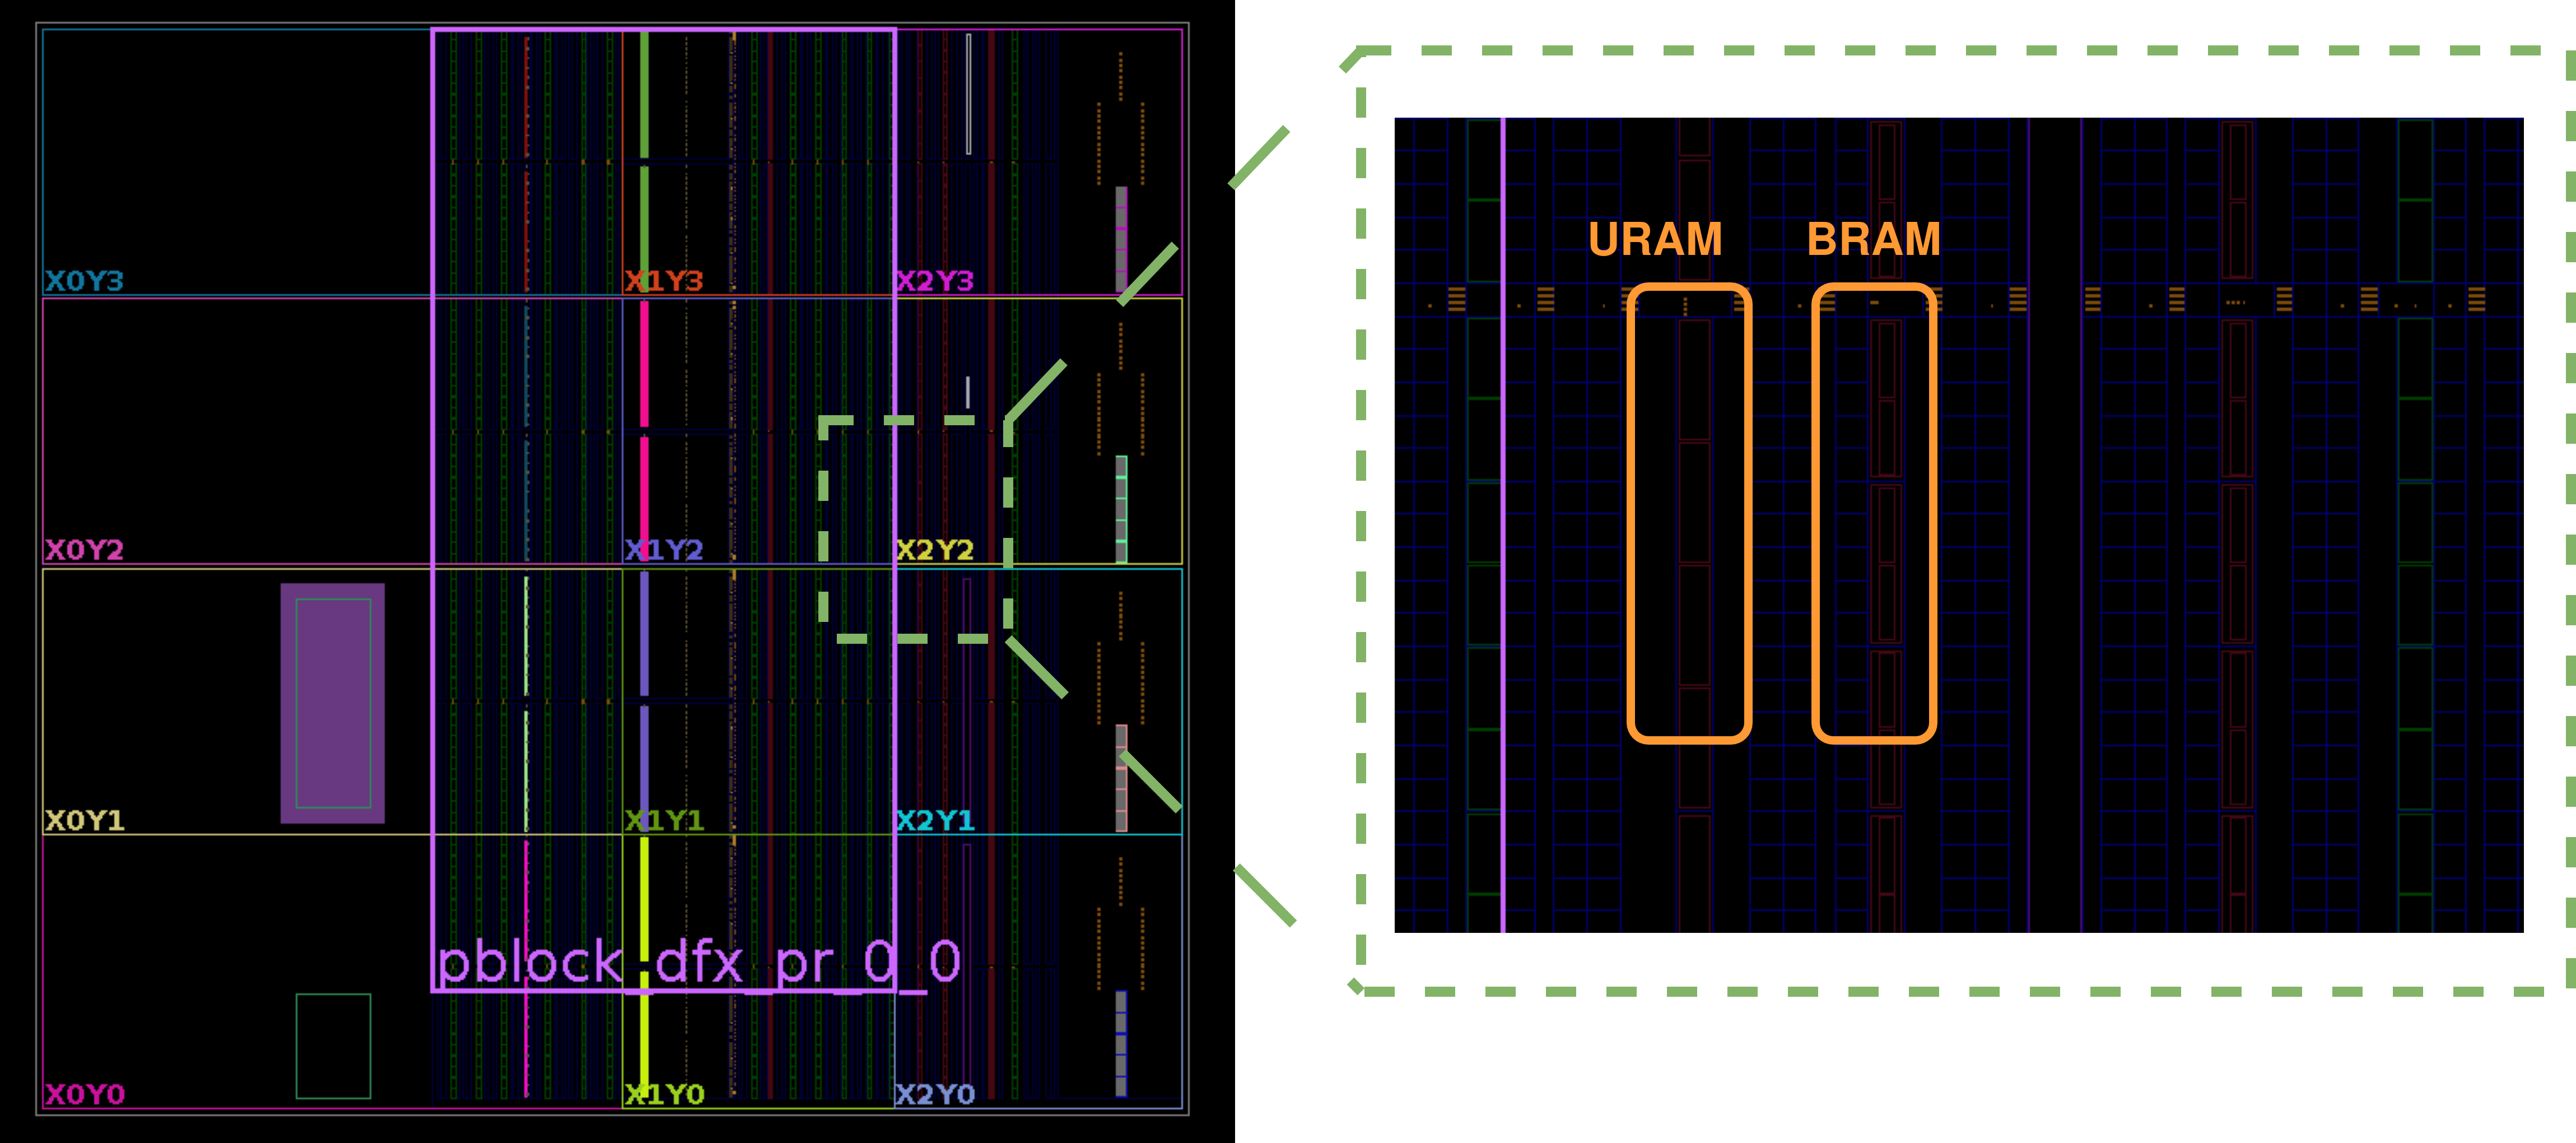
\includegraphics[width=0.85\linewidth]{packing_layout.png}
  \caption{DFX Streamer packing layout for the dynamic region.}
  \label{fig:packing_layout}
\end{figure}

\pagebreak 

\subsubsection{HLS4ML model}

We used the modified HLS4ML Vitis Unified Backend with the following ML model (image generated by Claude).

\begin{figure}[H]
  \centering
  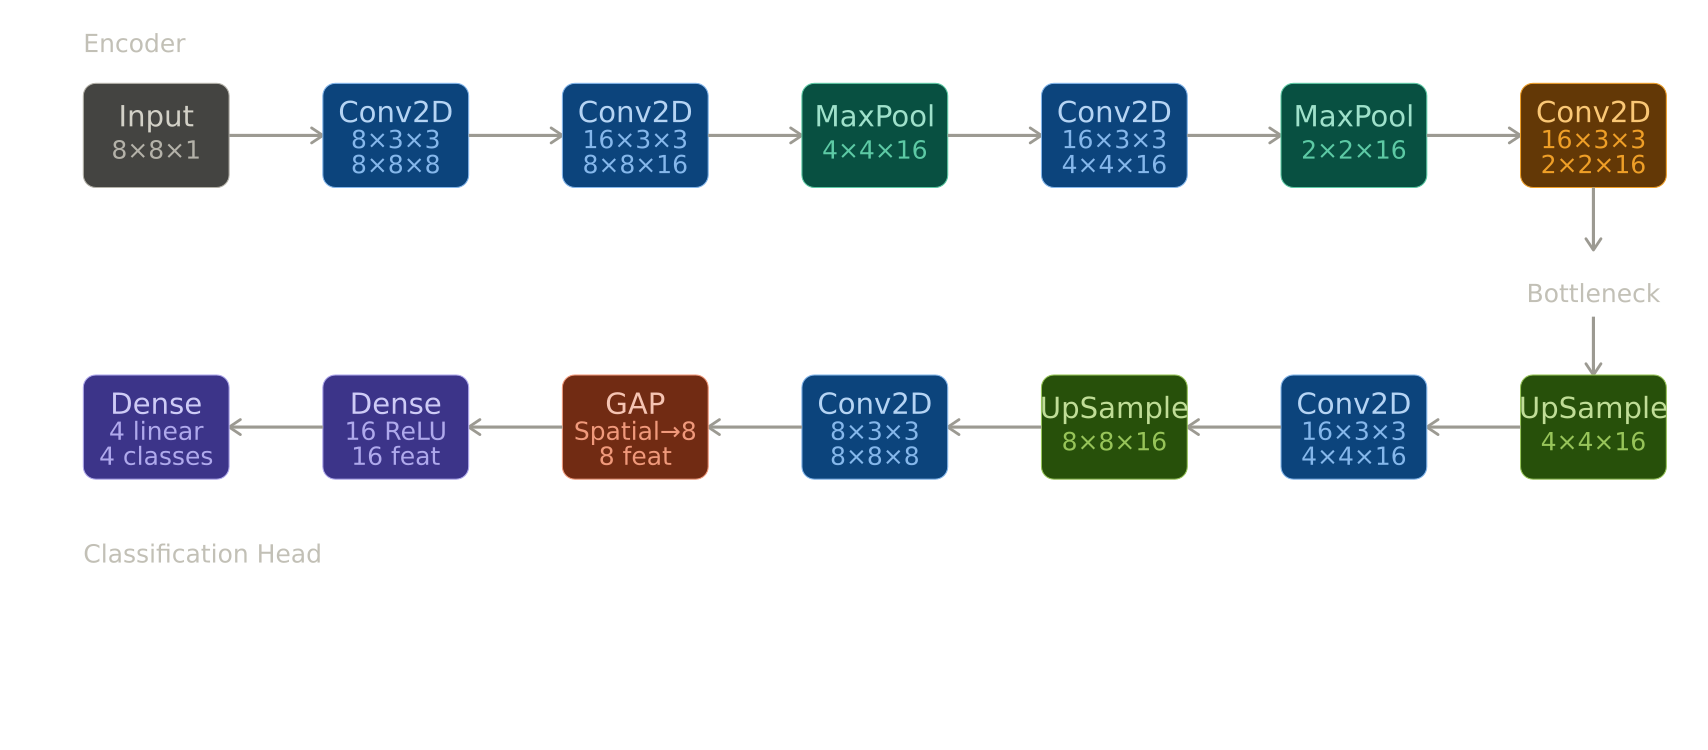
\includegraphics[width=0.85\linewidth]{ML.png}
  \caption{ML model architecture used in the experiment.}
  \label{fig:ml_model}
\end{figure}

The model generated code and debugger are at \url{https://github.com/Tanawin1701d/hls4ml/blob/VitisUnifiedPartialExp/simple_conv_nn_vitis_unified_exp.py}

The model was chopped at the bottleneck layer and the FIFO-depth optimisation was copied from the Vitis Unified Backend's model. The reuse factor was globally set to 8, although the internal HLS4ML logic may adjust it to match kernel alignment.

\begin{sloppypar}
In addition, we have modified the convolution to fix the BRAM over-utilisation problem for weight storage (\url{https://github.com/Tanawin1701d/hls4ml/commit/f21523ba25b67e429cc411d2b75378817aeb2cf4}).
\end{sloppypar}

In this model, the intermediate layer contains $(2 \times 2 \times 16)$ values at \texttt{ap\_fixed<16>}. The wavefront width of DFX Streamer (Magic Streamer) is therefore $16 \times 16 = 256$ bits, and each query requires 4 wavefronts ($2 \times 2$), giving a \textbf{query width of $4 \times 256 = 1024$ bits}.

The number of queries that can be packed into the available memory resources is calculated as follows:

\begin{align*}
\text{Query width} &= 2 \times 2 \times 16 \times 16\ \text{bits} = 1024\ \text{bits} \\[6pt]
\text{URAM288 queries} &= \frac{\text{blocks} \times \text{rows} \times \text{bit-width}}{\text{query width}}
  = \frac{64 \times 4096 \times 64}{1024} = 16384\ \text{queries} \\[6pt]
\text{BRAM36 queries}  &= \frac{\text{blocks} \times \text{rows} \times \text{bit-width}}{\text{query width}}
  = \frac{96 \times 512 \times 64}{1024} = 3072\ \text{queries}
\end{align*}

Therefore, we can pack approximately $16384 + 3072 = 19456 \approx 20000$ queries into DFX Streamer.
 



\subsubsection{Synthesis \& implementation}



\begin{figure}[H]
  \centering
  \begin{minipage}[t]{0.48\linewidth}
    \centering
    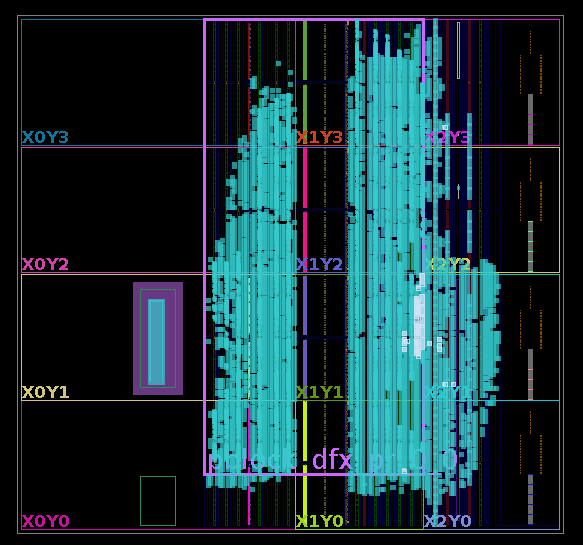
\includegraphics[width=\linewidth]{images/layout_config_0.png}
    \caption{Layout First Half.}
    \label{fig:layout_config_1}
  \end{minipage}
  \hfill
  \begin{minipage}[t]{0.48\linewidth}
    \centering
    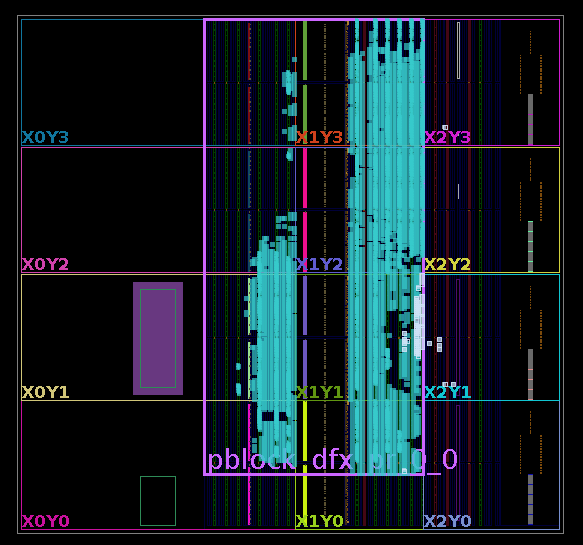
\includegraphics[width=\linewidth]{images/layout_config_1.png}
    \caption{Layout Second Half.}
    \label{fig:layout_config_2}
  \end{minipage}
\end{figure}

\begin{table}[H]
  \centering
  \caption{Implementation results: timing and hardware resource utilisation (KV260, xck26-sfvc784-2LV-c).}
  \label{tab:impl_results}
  \small
  \begin{tabular}{lrrrrrr}
    \toprule
    \textbf{Run} & \textbf{WNS (ns)} & \textbf{LUT} & \textbf{FF} & \textbf{BRAM} & \textbf{URAM} & \textbf{DSP} \\
    \midrule
    impl\_dfx           & 0.15 & 30{,}964 & 37{,}029 & 59 & 64 & 728 \\
    child\_2\_impl\_dfx & 0.70 & 27{,}256 & 33{,}511 & 59 & 64 & 480 \\ 
    \bottomrule
  \end{tabular}
\end{table} 





\subsubsection{Query Explore: Reconfiguration vs Execution Time}

The reconfiguration time is essentially constant across query counts (it depends only on bitstream
size), while the execution time grows linearly with the number of queries.
Each configuration is shown at full range alongside a zoomed view ($<5000$ queries). 

\subsubsection*{Configuration 1}

\begin{figure}[H]
  \centering
  \begin{minipage}[t]{0.54\linewidth}
    \centering
    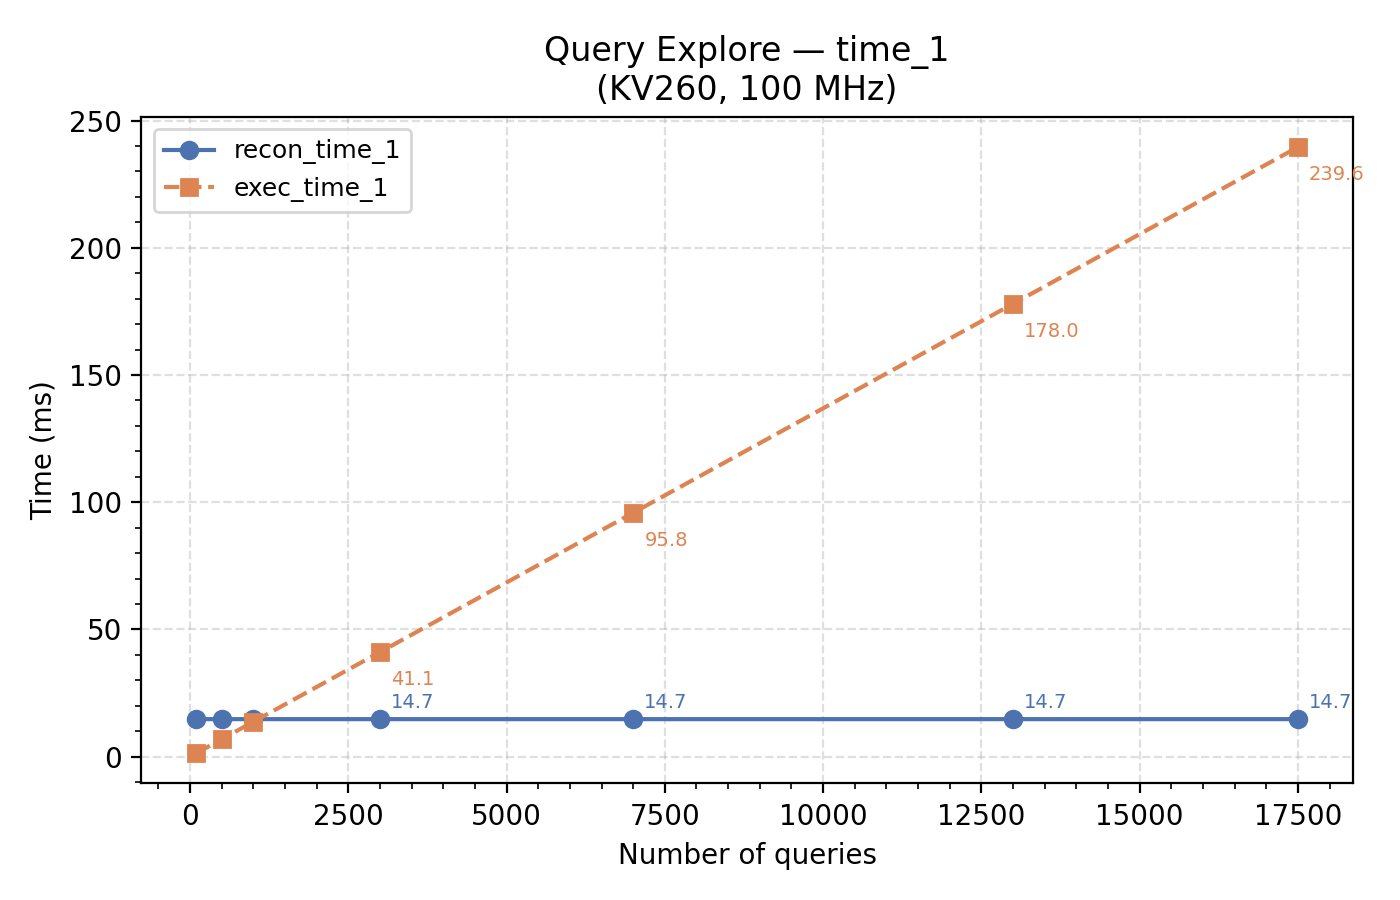
\includegraphics[width=\linewidth]{query_explore_time_1.png}
    \caption{Configuration~1 --- full range (KV260, 100\,MHz).}
    \label{fig:qe_time1}
  \end{minipage}
  \hfill
  \begin{minipage}[t]{0.44\linewidth}
    \centering
    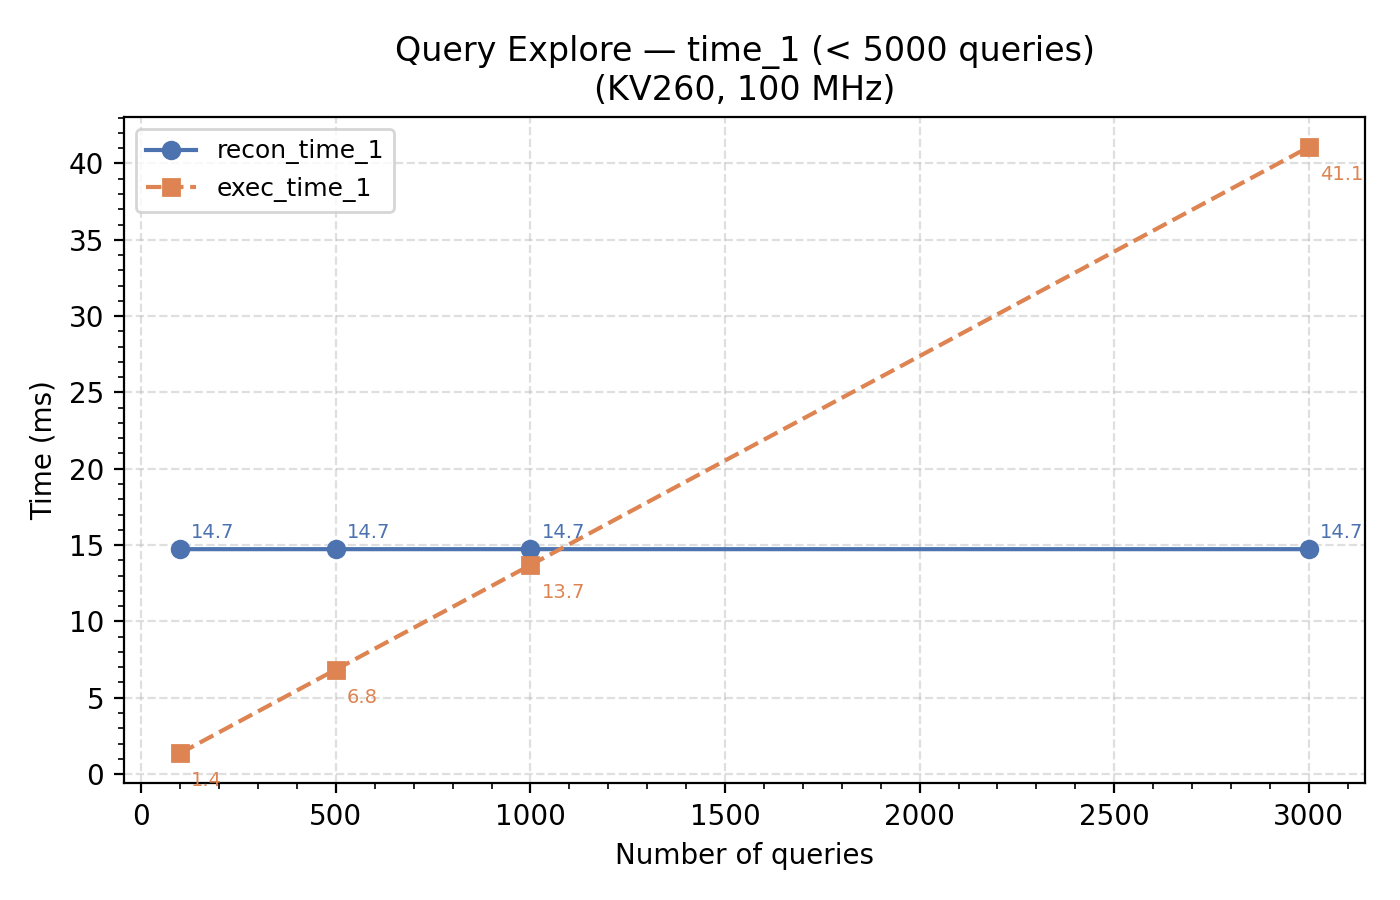
\includegraphics[width=\linewidth]{query_explore_time_1_zoom.png}
    \caption{Configuration~1 --- zoomed ($<5000$ queries).}
    \label{fig:qe_time1_zoom}
  \end{minipage}
\end{figure}

\subsubsection*{Configuration 2}

\begin{figure}[H]
  \centering
  \begin{minipage}[t]{0.54\linewidth}
    \centering
    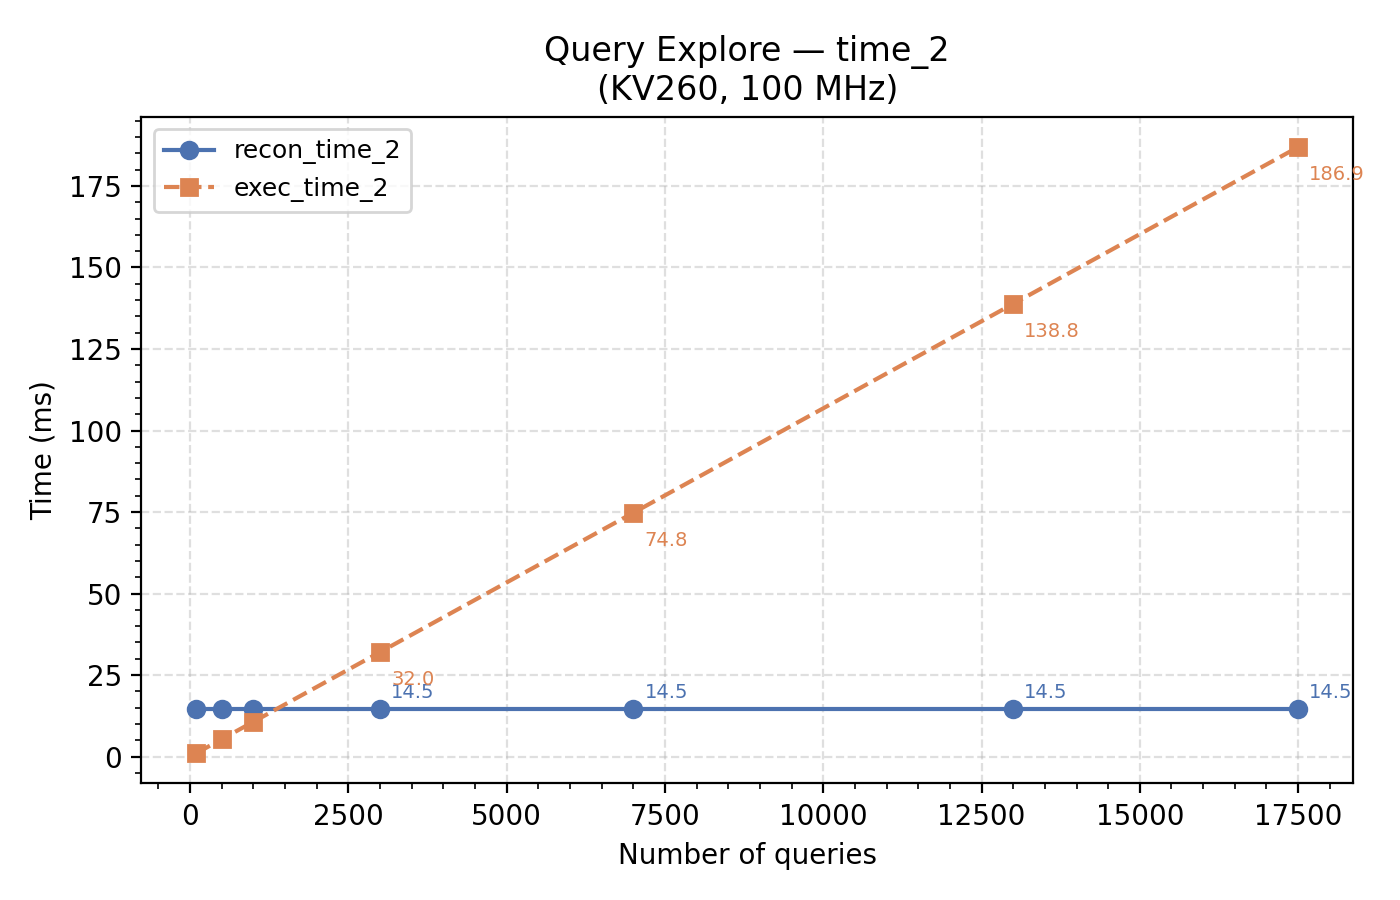
\includegraphics[width=\linewidth]{query_explore_time_2.png}
    \caption{Configuration~2 --- full range (KV260, 100\,MHz).}
    \label{fig:qe_time2}
  \end{minipage}
  \hfill
  \begin{minipage}[t]{0.44\linewidth}
    \centering
    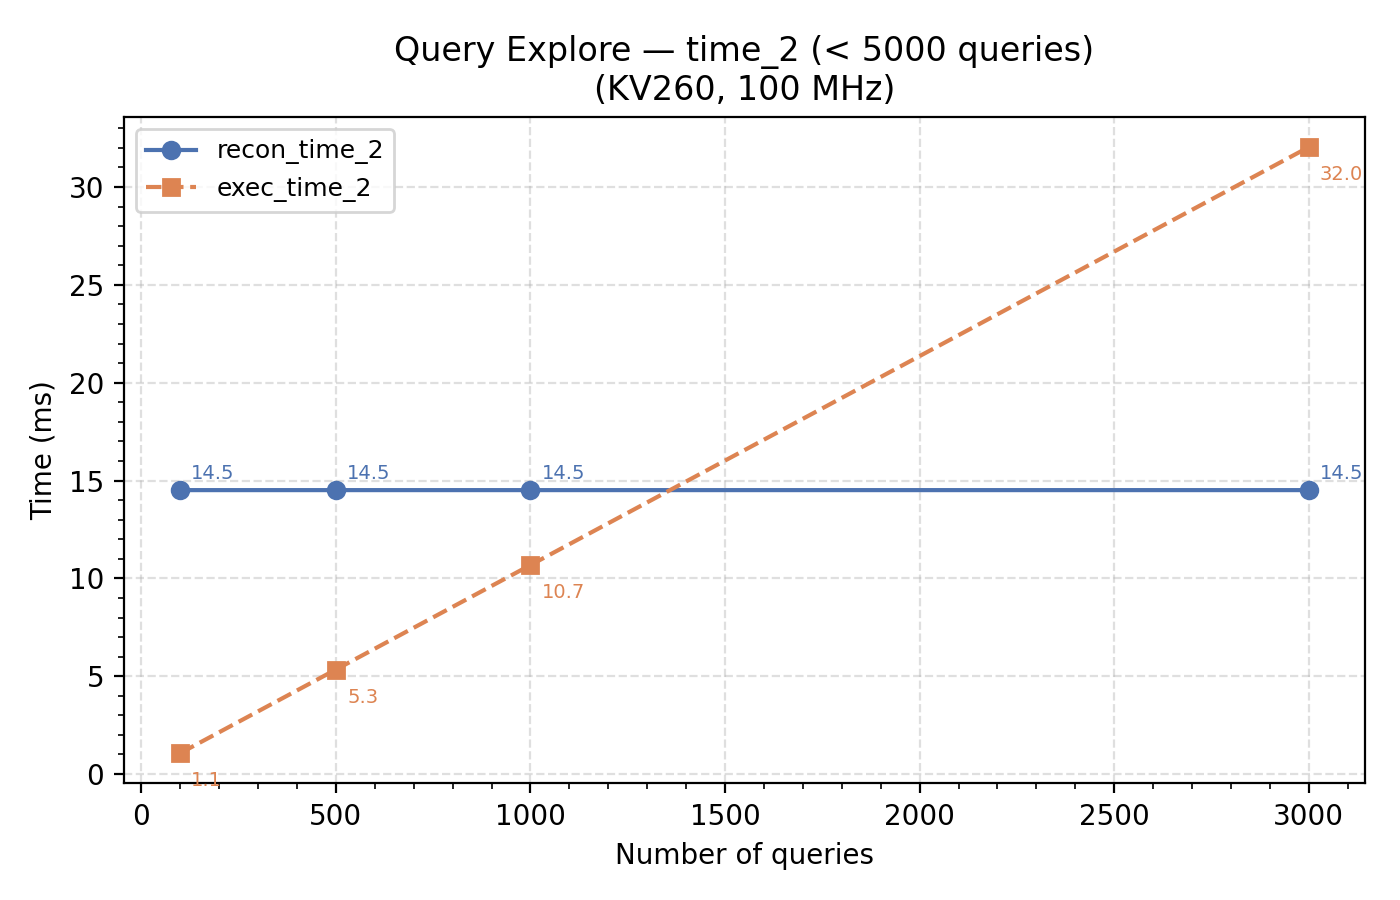
\includegraphics[width=\linewidth]{query_explore_time_2_zoom.png}
    \caption{Configuration~2 --- zoomed ($<5000$ queries).}
    \label{fig:qe_time2_zoom}
  \end{minipage}
\end{figure}

\pagebreak 

 

\subsection{Multi-Region (IN-PROGRESS)}

Before modifying the entire system to support multiple DFX regions, we would like to conduct a small experiment to understand how to work with multi-region configurations. The aspects we are considering include:

\begin{enumerate}
  \item DFX Ctrl IP:
  \begin{enumerate}
    \item Explore how to manage signals for multi-region configurations.
    \item Explore increasing the ICAP3 clock to 200\,MHz (the maximum recommended clock rate for ICAP3 on Zynq UltraScale+) to raise the transfer rate from $\sim$400\,MB/s to $\sim$800\,MB/s, while keeping the rest of the fabric at 100\,MHz (ML and static region).
  \end{enumerate}

  \item DFX Manager IP (Magic Sequencer):
  \begin{enumerate}
    \item We are considering upgrading bank 1 to support the latency hiding technique, but the architecture has not yet been finalised.
    \item The DFX Manager is currently large and difficult to maintain in Verilog; we may consider rewriting it in SystemVerilog. (I think Claude can do this perfectly.)
  \end{enumerate}

  \item Tcl Scripts (Block Design):
  \begin{enumerate}
    \item We need to upgrade the Tcl scripts to enable multi-region connections and DFX Streamer arrangement.
  \end{enumerate}

\end{enumerate}


\end{document}


